\documentclass[a4, 12pt, addpoints]{exam}
\usepackage[margin=0.9in, top = 2cm]{geometry}
\usepackage[utf8]{inputenc}
\usepackage{graphics}
\usepackage{color}
\usepackage{amssymb}
\usepackage{amsmath}
\usepackage{enumitem}
\usepackage{xcolor}
\usepackage{cancel}
\usepackage{ragged2e}
\usepackage{graphicx}
\usepackage{multicol}
\usepackage{color}
\usepackage{tikz}
\usepackage{circuitikz}
\usepackage{siunitx}
\usepackage{longtable}
\usepackage{float}
\usepackage{parskip}
\usepackage{caption, subcaption}
\CorrectChoiceEmphasis{\itseries\color{red}}

\runningfooter%
    {}
    {\textbf{D.I.E.T., Satara}}
    { \thepage
    %\iflastpage{}{
%        \textbf{Question \thequestion }%
%        \ifcontinuation{ -- continued}{}\\%
%        \oddeven{\textbf{TURN OVER}}{}
%        }
    }
%MOVE THIS FOOTER TO THE RIGHT BY 0.4in, same for the header, but I've left it out as the header is even longer which lots of if conditions.

\pagestyle{headandfoot}
\begin{document}
\def\arraystretch{1}
\begin{longtable}{lp{0.65\textwidth}p{0.15\textwidth}r}
\multicolumn{4}{c}{
\includegraphics[width= \textwidth]{dietlogo}} \\ 
\multicolumn{4}{c}{Written Test for Degree Engineering Interview} \\
Date: 20/07/2024 & \multicolumn{2}{c}{Time:1 hr} & Marks:20 \\
\multicolumn{4}{l}{ Note: All questions are carry equal marks} \\ \hline
\end{longtable}
%\vspace{0.1in}
\begin{questions}
\question If silicon diode is operating in forward bias in a circuit with 12 V supply and 240 $\Omega$ series resistance, then what is the voltage drop across the diode. \\[0.3cm]
\begin{oneparchoices}
\choice 1.5 V
\choice 0.4 V
\choice 1.1 V
\choice 0.7 V
\end{oneparchoices}  
\question In feedback control system shown in Figure~\ref{q2} below $ G(s) = \dfrac{6}{s(s+1)(s+2)} $, where $R(s), Y(s), \& E(s)$ are Laplace transform of $r(t), y(t), \& e(t) $ respectively, if the input $r(t)$ is a unit ramp function then ------  \\[0.3cm]
\begin{figure}[h!]
\centering
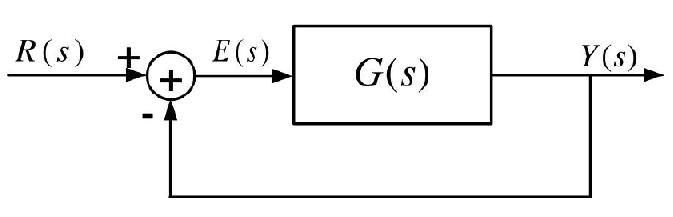
\includegraphics[width=0.5\textwidth]{fbc.png}
\caption{Q.No.2}
\label{q2}
\end{figure}
\begin{oneparchoices}
\choice $\lim \limits_{t \to \infty } e(t) = 0$
\choice $\lim \limits_{t \to \infty } e(t) = \dfrac{1}{3}$
\choice $\lim \limits_{t \to \infty } e(t) = \dfrac{1}{4}$
\choice $\lim \limits_{t \to \infty } e(t) $ does not exist, $e(t)$ is oscillatory.
\end{oneparchoices}  
\question What is the z-transform of the following finite duration signal? $ x[n] = \{ 2, 4, \underset{\uparrow}{5}, 7, 0, 1 \} $\\[0.3cm]
\begin{oneparchoices}
\choice $ 2 + 4z + 5z^2 + 7z^3 + z^4  $
\choice $2 + 4z + 5z^2 + 7z^3 + z^5$
\choice $ 2 + 4z^{-1} + 5z^{-2} + 7z^{-3} + z^{-5} $
\choice $ 2z^2 + 4z + 5 +7z^{-1} + z^{-3}$
\end{oneparchoices}  
\question The BJT as a switch is is operated in one of the following:
\begin{oneparchoices}
\choice Only saturation region
\choice Active region
\choice Only cut off region
\choice Both saturation and cut off region
\end{oneparchoices}  
\question A DC power supply has no load voltage of 30 V and full load voltage of 25 V at full load current of 1 A. Its output resistance and load regulation respectively are. \\[0.3cm]
\begin{oneparchoices}
\choice $5 \Omega$ and $20 \%$ 
\choice $25 \Omega$ and $20 \%$
\choice $5 \Omega$ and $ 16.7 \%$
\choice $25 \Omega$ and $16.7 \%$
\end{oneparchoices} 
\question A 500 W carrier signal is amplitude modulated modulation percentage of 60\%.  The total power in the modulated signal if the form amplitude modulation used is  the double sideband AM with full carrier(A3E). \\[0.3cm]
 \begin{oneparchoices}
\choice 590 W
\choice 534 W
\choice 125 W
\choice 300 W
\end{oneparchoices} 
\question What will be the o/p of the given logic gate of Figure~\ref{lg}?
\begin{figure}[H]
\centering
\resizebox{0.38\textwidth}{!}{
\begin{circuitikz}[american voltages]
\draw
 
 (0,2) node[nor port] (mynor1) {}
(0,0) node[nor port] (mynor2) {}
(2,1) node[nor port] (mynor) {}
(mynor1.out) -- (mynor.in 1)
(mynor2.out) -- (mynor.in 2)
(4,1) node[nor port] (mynor3) {}
(mynor3.west) -- (mynor.out)
(mynor3.in 1) -- (mynor3.in 2)
(mynor1.in 1) -- (mynor1.in 2)
(mynor2.in 1) -- (mynor2.in 2)
(mynor1.west) -- (-2,2)
(mynor2.west) -- (-2,0)
(-2.2,2) node{A}
(-2.2,0) node{B}
(mynor3.east) node {~~~Q} ;  
\end{circuitikz}}
\caption{Q.No.7}
\label{lg}
\end{figure}
\begin{oneparchoices}
\choice NOR
\choice NAND
\choice AND
\choice OR
\end{oneparchoices} 
\question Let $\hat{i}$ and $\hat{j}$ be the unit vectors along $x$ and $y$ axes respectively, and let $A$ be the positive constant. Which one of the following is true for vector fields $ \bar{F_1} = A ( \hat{i} y + \hat{j} x ) $, $ \bar{F_2} = A ( \hat{i} y - \hat{j} x ) $  \\[0.3cm]
\begin{oneparchoices}
\choice Both $\bar{F_1}$ and $\bar{F_2}$ are electrostatic fields.
\choice Only $\bar{F_1}$ is an electrostatic fields.
\choice Only $\bar{F_2}$ is an electrostatic fields.
\choice Neither $\bar{F_1}$ nor $\bar{F_2}$ are electrostatic fields.
\end{oneparchoices} 
\question The current $I_y$ flowing through $660 \Omega$ resistance  is (Refer Figure~\ref{fig:1}):
\begin{figure}[H]
\centering
\resizebox{0.35\textwidth}{!}{
\begin{circuitikz}[american voltages]
\draw
(0,4) to [V, v_= $3V$, i = $I_x$] (0,0);
\draw
 (0,4)     to [short]      (3,4)
      to [R, i= $I_y$, l=$660 \Omega$] (6,4);
\draw
(0,0) to [R, l=$330\Omega$] (3,0);
\draw
(3,4) to [short] (3,3)
      to [R, l=$660\Omega$] (6,3)
      to [short] (6,4);
\draw
(6,3) to [short] (3,0)
      to [R, l_=$330 \Omega$] (0,4);      
\end{circuitikz}}
\caption{Q.No.9}
\label{fig:1}
\end{figure}

\begin{oneparchoices}
    \choice $I_x$
    \choice $I_x/2$
    \CorrectChoice $I_x/4$
    \choice $I_x/3$
\end{oneparchoices}

\question In the circuit shown below, P and Q are the inputs. The logical function realized by the circuit shown Figure~\ref{fig:2} below is:
\begin{figure}[H]
\centering
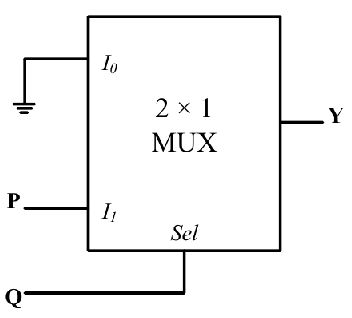
\includegraphics[width=0.25\textwidth]{mux}
\caption{Q.No.10}
\label{fig:2}
\end{figure}
\begin{oneparchoices}
    \choice $Y = PQ$
    \choice $Y=P+Q$
    \choice $Y = \overline{PQ}$
    \CorrectChoice $Y= \overline{P + Q}$
    
\end{oneparchoices}



\vspace{0.10in}

\end{questions}
\end{document}
 